\documentclass[11pt,a4paper,headings=small,dvips]{scrbook}

\input{configuration.tex}

\begin{document}

\setcounter{page}{1}

\begin{titlepage}
	\title{ \textcolor{blue01}{\textsf{\bfseries\Huge NHLIB}}  }
	\date{May 2012}
	\publishers{GEM Foundation, Pavia}
\end{titlepage}
\pagestyle{scrheadings}
\maketitle

\renewcommand*\thesection{\arabic{section}}
\renewcommand*\thefigure{\thesection.\arabic{figure}}
\renewcommand*\thefigure{\thesubsection.\arabic{figure}}

\section{Introduction}
\setcounter{figure}{0}
NHLIB ( `New Hazard LIBrary' -- https://github.com/gem/nhlib), is the python-based library designed to power the seismic hazard module of the OpenQuake platform. It provides tools for modeling seismogenic sources (as points, areas and faults), earthquake ruptures, temporal (e.g. Poissonian) and magnitude occurrence models (e.g. Gutenberg-Richter), magnitude/area scaling relationships, ground motion and intensity prediction equations (i.e. GMPEs and IPEs). It currently offers an hazard curve calculator, and as the development continues, it will provide calculators for stochastic event sets, ground motion fields and disaggregation histograms.\\
NHLIB has been designed to provide efficient and optimized PSHA calculators to reduce computation time and memory (i.e. RAM) usage as much as possible. Long computation times may often force undesired simplifications in the input model, only with the purpose of obtaining results in a reasonable time, while large memory consumption put strong constrains on the system hardware the software requires and therefore limits its usability.\\
Since the very beginning, NHLIB has been created following the `Test Driven Development', which makes the software not only verified in its different components, but also placed in a controlled environment, which allows further developments/optimizations to happen under safe conditions, reducing the risk of introducing defects or errors.\\
Being python-based, NHLIB allows an easier integration in the OpenQuake platform, again facilitating the development and simplifying the system architecture.\\
The present document aims at describing the NHLIB main features: the modeling of seismogenic sources (section \ref{source_modeling}), the implementation of ground shaking intensity models (i.e. GMPEs and IPEs, section \ref{gsim}) and the currently implemented hazard curve calculator (section \ref{hcc}). Validation of the library for few selected cases is done through the PEER tests (\cite{thomas2010}, reported in section \ref{peer}). Section \ref{performances} describes NHLIB performances, while section \ref{conclusions} summarizes the current state of the library and the development planned for the next future.\\

\section{Source Modeling}\label{source_modeling}
\setcounter{figure}{0}
In the context of NHLIB, the term `Source Modeling' indicates the process by which primary seismogenic source data (e.g. source geometry, activity rates, faulting style, hypocenter depth distribution) are used to construct the inventory of all possible earthquake ruptures in a region of interest, together with their probability of occurrence; that is the `Earthquake Rupture Forecast' (\cite{field2003}).\\
OpenQuake currently defines four source typologies (\cite{crowley2011}): point, area, simple fault, and complex fault. These four types have been identified by analyzing different PSHA models developed for different parts of the world (\cite{pagani2010}). \\
The following sections describe the NHLIB implementation of the different source typologies. Each source typology  is defined by a set of parameters, which reflect the different types of data/information required to create a seismogenic source for PSHA. Apart from the source specific parameters, each source is defined by the following common parameters:
\begin{itemize}
\item ID
\item NAME
\item TECTONIC REGION TYPE
\item MAGNITUDE FREQUENCY DISTRIBUTION
\item MAGNITUDE SCALING RELATIONSHIP
\item RUPTURE ASPECT RATIO
\item RUPTURE MESH SPACING
\end{itemize}
The ID and name parameters offers way for selecting and identifying each source, while the tectonic region type defines the tectonic regime the source belongs to. This information is required to map each seismogenic source to the appropriate equation for predicting ground shaking (see section \ref{hcc}). This is consistent with the current practice of defining GMPEs or IPEs that are tectonic region dependent (e.g. \cite{zhao2006}, \cite{campbell2003SCR}). The magnitude frequency distribution defines the distribution of earthquakes occurrence rates over magnitude, and basically determines the energy released by a source. The magnitude scaling relationship, rupture aspect ratio and mesh spacing are the required parameters for modeling earthquake ruptures. Each source typology models earthquake ruptures as 3D surfaces, so the scaling relationship allows to derive rupture area from rupture magnitude, while the aspect ratio (rupture length/ rupture width) allows the definition of the rupture shape. Each earthquake rupture has, by default, a mesh representation, the resolution of the mesh being determined by the mesh spacing (expressed in km).\\
Currently, rupture area is computed as the median area provided by the scaling relationship given magnitude, and if considered, rake values. However, the NHLIB scaling relationship can provide also the standard deviation of the area distribution, as well as area values affected by an uncertainty term (specified as an $\epsilon$ value). This open the possibility to include aleatory uncertainties associated to a scaling relationship in the rupture modeling -- that is to consider multiple ruptures associated to the same magnitude value, but having different areas, and with occurrence rates scaled accordingly to the areas' probabilities (as given by the scaling relationship).\\
It is worth noting that in the NHLIB data model the magnitude scaling relationship and aspect ratio are source properties (to honor the fact that rupture size may depend on tectonic region and rupture shape my depend on faulting style), while in the current OpenQuake engine scaling relationship and aspect ratio are defined per source typology and therefore considered more as `calculation parameters'.\\

\subsection{Point and Area sources}
\setcounter{figure}{0}
A `Point Source' represents seismicity occurring on a single geographical location, while an `Area Source' represents uniform seismicity occurring over a polygonal geographical region.  Both point and area sources are often used to describe seismicity that cannot be associated to known or well constrained fault structures.\\
In NHLIB, point and area sources are described by the following common parameters:
\begin{enumerate}
\item UPPER SEISMOGENIC DEPTH
\item LOWER SEISMOGENIC DEPTH
\item NODAL PLANE DISTRIBUTION
\item HYPOCENTER DEPTH DISTRIBUTION
\end{enumerate}
The upper and lower seismogenic depths represent the minimum and maximum depths an earthquake rupture can reach, respectively. This information is required to constrain earthquake ruptures to occur over the depth range for which the source is defined. The nodal plane distribution defines a probability mass function for the ruptures nodal planes (each nodal plane being defined by the three angles: strike, dip, rake). This allows to define, in the same source, multiple faulting styles or multiple rupture orientations. For each rupture, the original rate is scaled according to the probability/weight associated to the corresponding nodal plane. Similarly, the hypocenter depth distribution defines a probability mass function for the ruptures' hypocenter depths allowing therefore multiple rupture nucleation depths in the same source (again rupture rates are scaled according to the corresponding hypocenter depth weight).\\
In a point or area source, earthquake ruptures are modeled as 3D planar rectangles. Even if a mesh representation can be computed, for calculation purposes the rupture plane is represented only by the coordinates of the four corners (and all distance calculations make use of this information only). The plane is initially centered at the hypocenter location, and the rupture extension along length and width is obtained by the rupture area (derived from the scaling relationship) and the given aspect ratio. If the resulting rupture plane width cannot be accommodated by the seismogenic layer thickness, the rupture plane is reshaped, and a new length is computed assuming the rupture extending for the entire seismogenic layer along dip. If, on the contrary, the rupture width can be accommodated by the seismogenic layer thickness, but because of the hypocenter location, the resulting plane extends above the upper seismogenic depth, then the plane is shifted downwards so that the top edge of the plane is located at the upper seismogenic depth. Similarly, if the rupture plane extends below the lower seismogenic depth, the plane is shifted upwards so that the bottom edge of the plane is located at the lower seismogenic depth. This mechanism is illustrated in Figure \ref{fig:ptSrc}.
\begin{figure}[htbp]
\centering
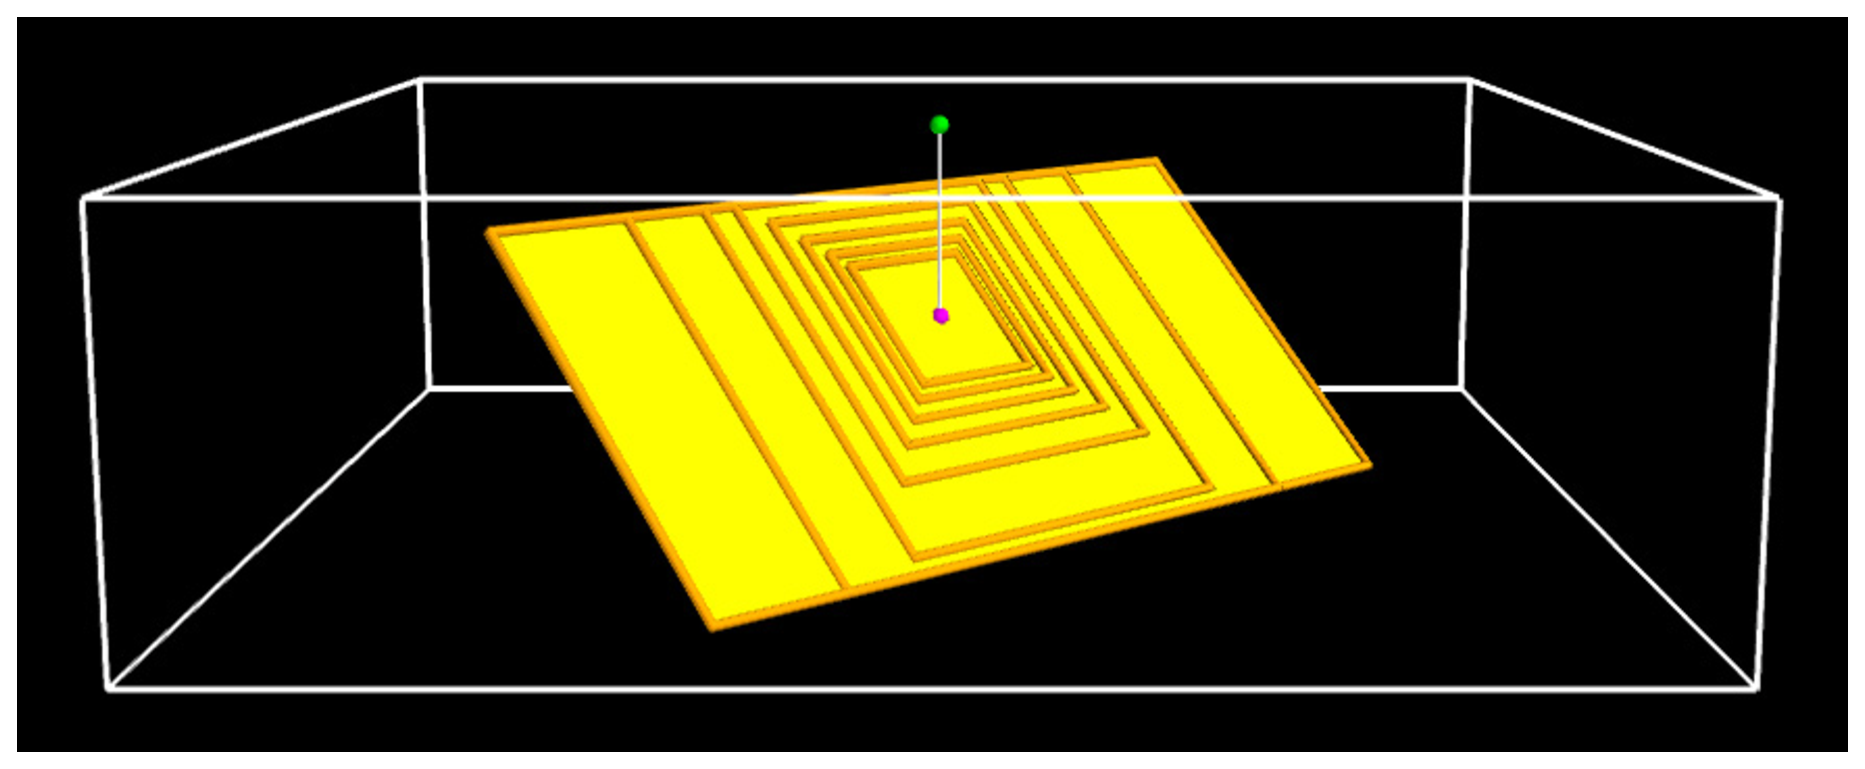
\includegraphics[width=12cm]{./figures/pointSource.eps}
\caption{Ruptures in a point source with single hypocentral depth and single nodal plane. Given a geographical location at the earth surface (green dot), ruptures (yellow planes) are generated and initially centered around the hypocenter (purple dot). Ruptures are progressively shifted downwards or reshaped so as to fit within the seismogenic layer. Minimum magnitude is 5.0, maximum magnitude is 6.5.}
\label{fig:ptSrc}
\end{figure}
\begin{figure}[htbp]
\centering
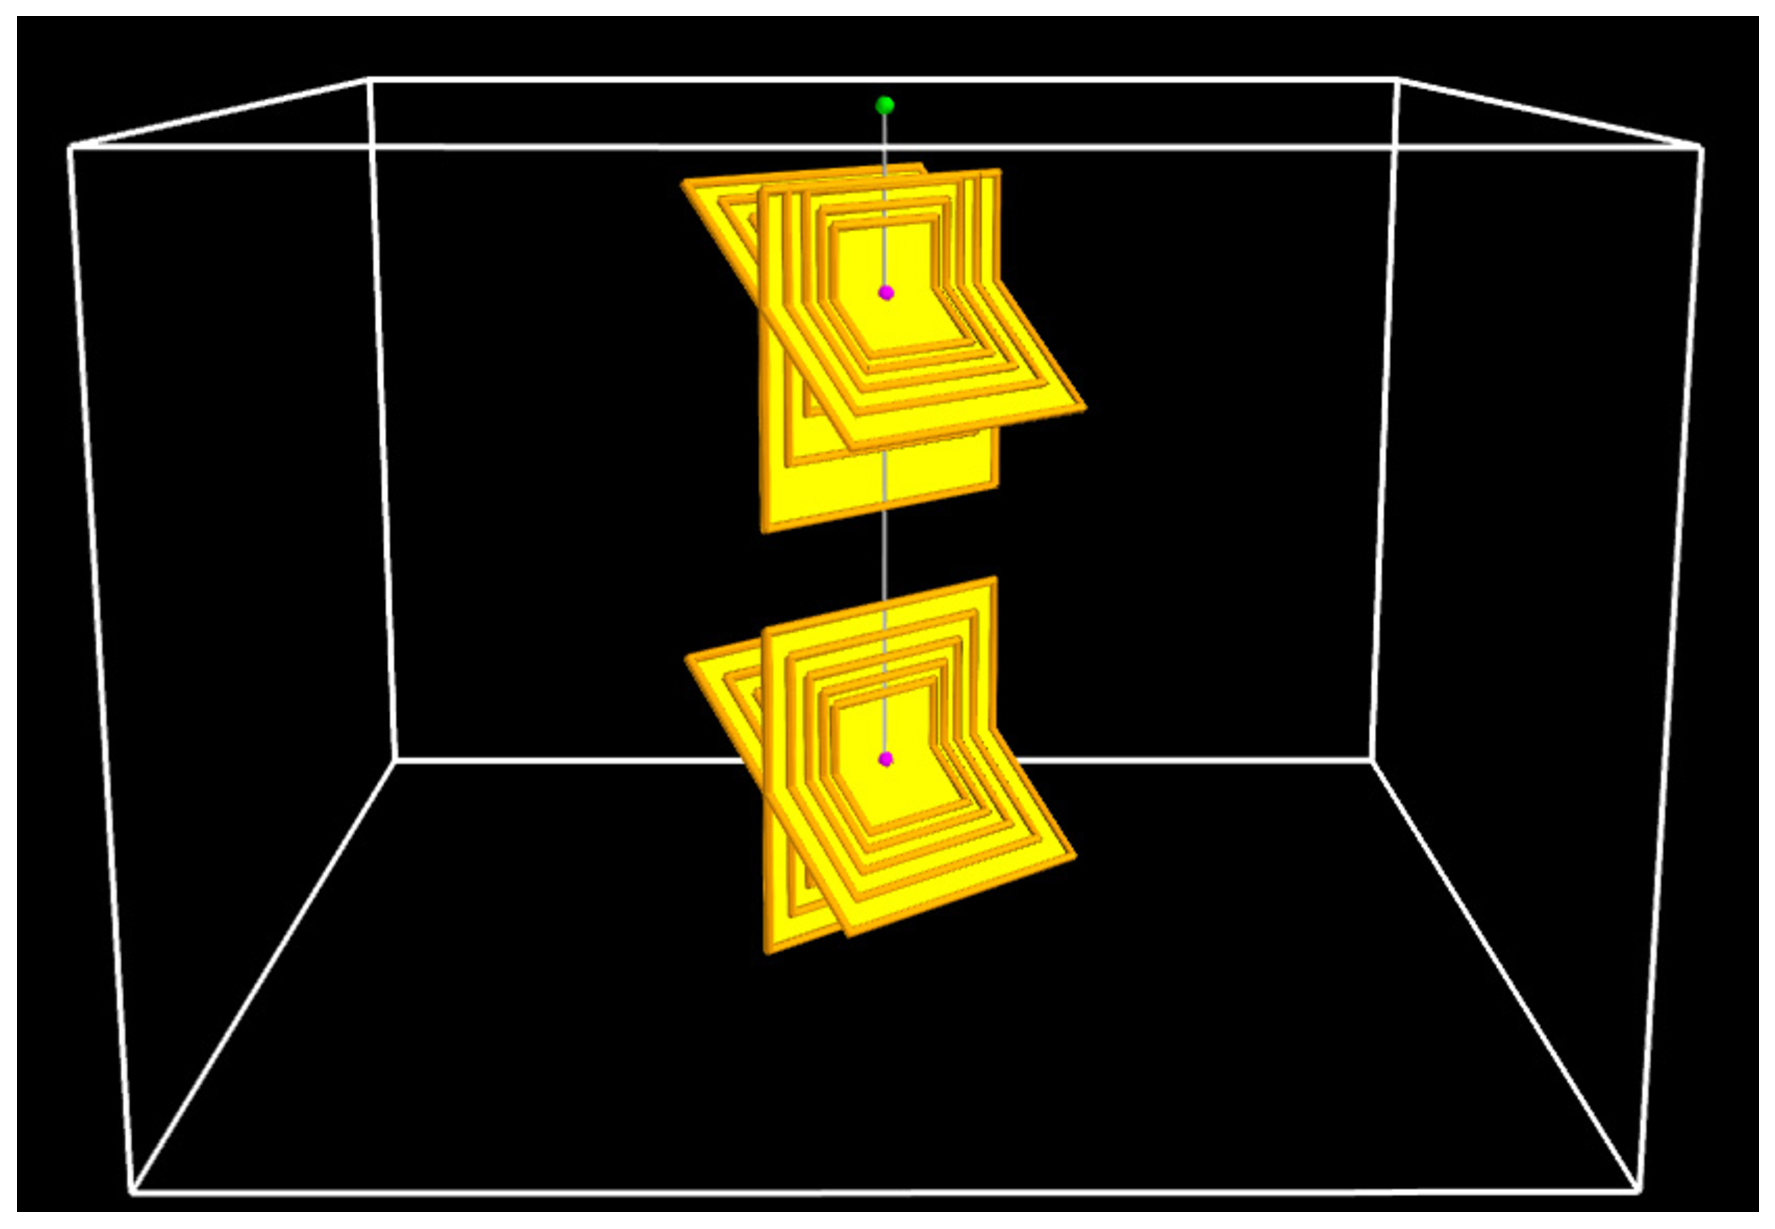
\includegraphics[width=12cm]{./figures/pointSourceMultiDepthsNodalPlanes.eps}
\caption{Ruptures in a point source with two hypocentral depths and two nodal planes (same strike but different dip: 45 and 90). Minimum magnitude is 5.0, maximum magnitude is 6.0.}
\label{fig:ptSrcMultiDepthsNodalPlanes}
\end{figure}
\begin{figure}[htbp]
\centering
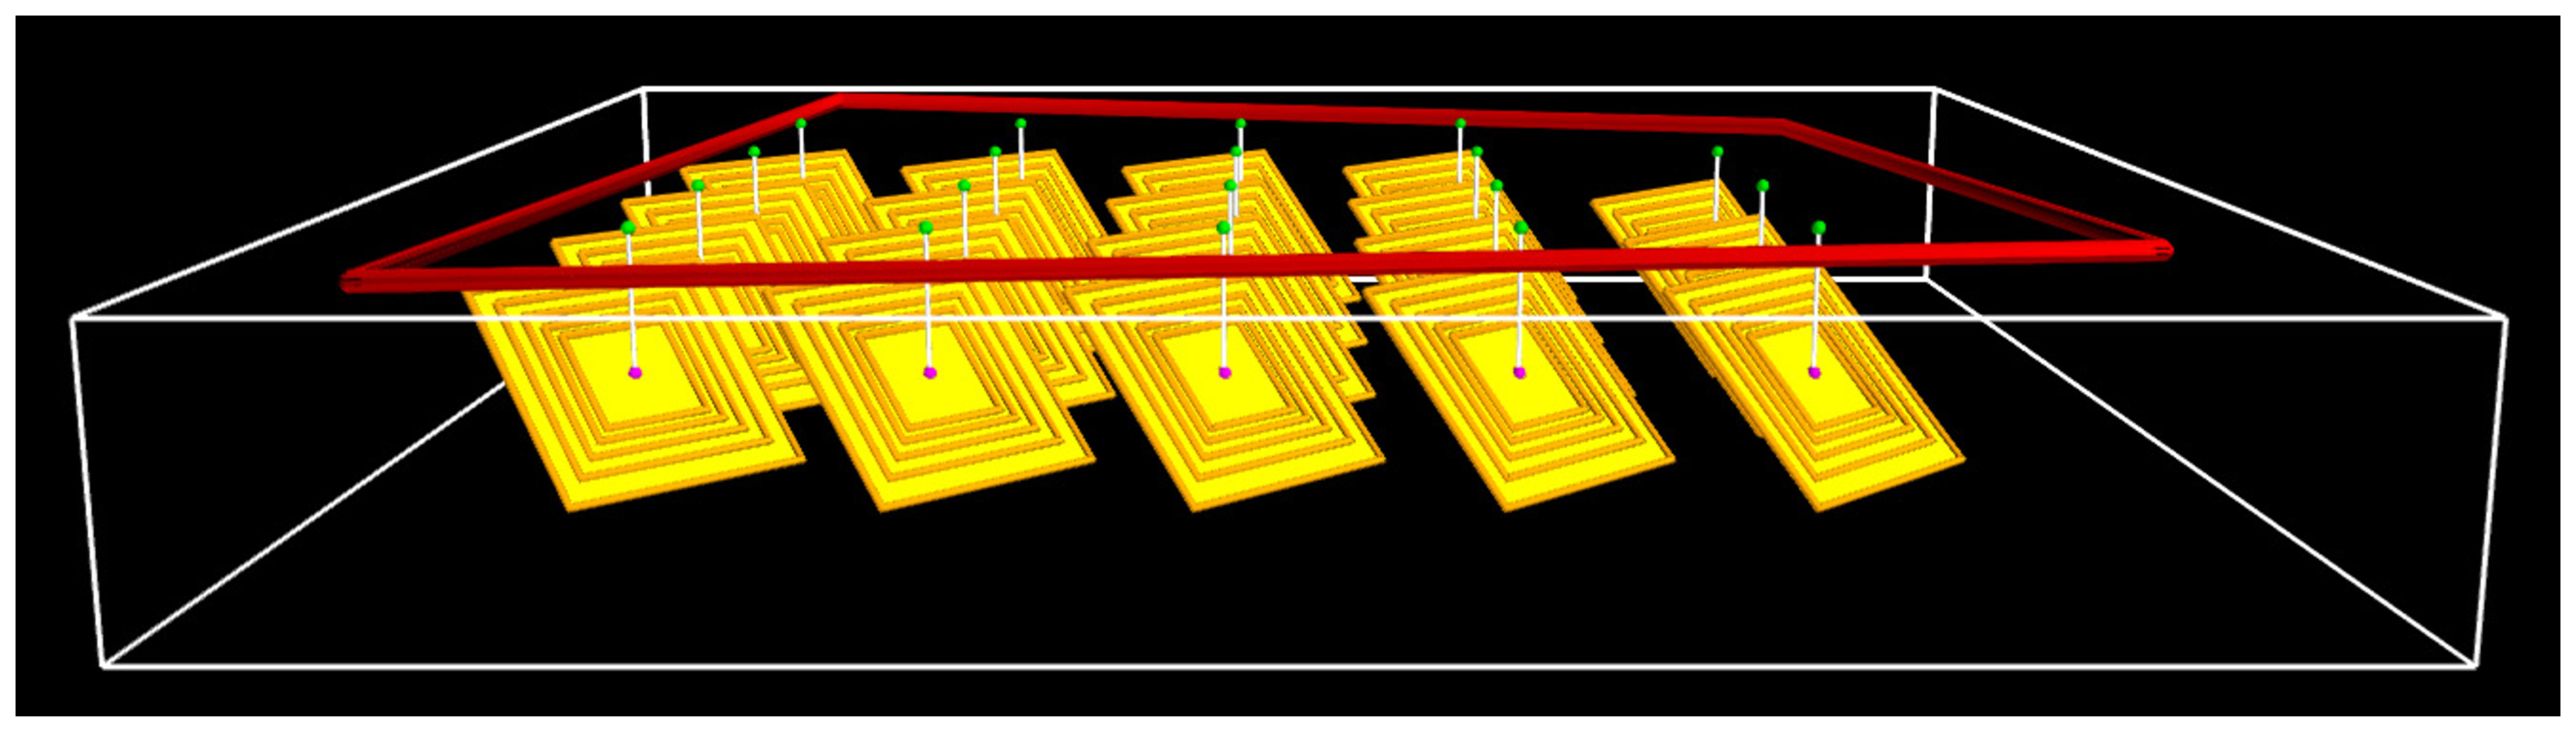
\includegraphics[width=12cm]{./figures/areaSrc.eps}
\caption{Ruptures in an area source (the red line represents the area boundary) with single hypocentral depth and single nodal plane. Rupture hypocenters are distributed over a uniform grid within the area boundary. Minimum magnitude is 5.0, maximum magnitude is 6.0.}
\label{fig:areaSrc}
\end{figure}
The figure shows earthquake ruptures as generated by a point source, having minimum magnitude equal to 5.0 and maximum magnitude of 6.5. The scaling relationship is Wells and Coppersmith 1994 (\cite{wells1994}), and the aspect ratio is set to 1. Ruptures are computed every 0.2 magnitude units. The upper seismogenic depth is set at 2.0 km and the lower seismogenic depth is set at 10.0 km. The hypocenter is defined at 5.0 km. Only one nodal plane is considered (with dip = 45). Low magnitude ruptures have a square shape (as expected from aspect ratio equal to 1), but as the size increases, ruptures are progressively shifted downwards until the bottom edge is reached, and therefore ruptures start to extend along length.\\
By having the possibility to define a nodal plane and hypocentral depth distributions, ruptures in a point or area sources can be distributed over different depths and have multiple orientations. Figure \ref{fig:ptSrcMultiDepthsNodalPlanes} illustrate such a situation. 
In this case the point source has a minimum magnitude equal to 5.0 and maximum magnitude equal to 6.0. The upper and lower seismogenic depths are 2.0 km and 22.0 km, respectively. Two hypocenter depths are defined (5.0 km and 18.0 km) and two nodal planes having the same strike angle but two different dip angles (45 and 90). By defining more nodal planes associated to different strike angles, it is also possible to define ruptures oriented according to multiple azimuths -- a useful approach in case a predominant faulting direction cannot be identified.\\
While the surface projection of the ruptures' hypocenters from a point source are concentrated on a single location, ruptures in an area source are distributed over a uniformly spaced mesh within the area boundary (see Figure \ref{fig:areaSrc}) and the occurrence rates are distributed evenly among all the nodes.

\subsection{Simple and Complex Fault sources}
\setcounter{figure}{0}
Fault sources are designed for modeling seismicity associated to fault structures for which activity rates can be estimated. Fault sources are usually used in PSHA to model crustal faults or to model large subduction interface events. The amount of data available to constrain a fault source may vary, therefore NHLIB provides two basic fault source typologies, which cope with different levels of complexity in the fault definition.\\
A `Simple Fault Source' is designed to model seismicity occurring on a fault structure that is characterized, as the name suggests, by a simple geometry. A simple fault source is defined by the following parameters:
\begin{itemize}
\item UPPER SEISMOGENIC DEPTH
\item LOWER SEISMOGENIC DEPTH
\item FAULT TRACE
\item DIP
\item RAKE
\end{itemize}
The upper and lower seismogenic depths again constrain the minimum and maximum depths an earthquake rupture can reach. The fault trace is defined as the intersection of the fault plane with the Earth surface. The dip angle defines the inclination of the fault plane with respect to the surface, and the rake angle is a property of the fault ruptures which reflect the faulting style (e.g. normal, reverse, strike-slip).\\
NHLIB represents a fault surface as a regular, that is uniformly spaced, 3D mesh of points. The fault surface is obtained by translating the fault trace along a direction that is perpendicular to the fault trace strike (computed as the azimuth between the first and last points in the trace), from the upper seismogenic depth to the lower seismogenic depth, following an inclination equal to the dip angle. The resulting surface is in general a non planar parallelogram. Figure \ref{fig:simpleFaultSrc1} shows an example of simple fault source, as derived by a fault trace, and considering an upper seismogenic depth of 2 km, a lower seismogenic depth of 20 km and a dip value equal to 60 degrees.\\
Ruptures are defined as portions of the fault surface (whose dimensions are derived from scaling relationship and aspect ratio), and placed over the entire fault surface, along strike and dip, with an offset that is equal to the rupture mesh spacing.\\
A `Complex Fault Source' allows to represent a more irregular fault surface geometry by defining a set of fault edges, consisting of at least the fault top and bottom edges, and, if available, a number of intermediate edges.The parameters required to define a complex fault source are therefore:
\begin{itemize}
\item FAULT TOP EDGE
\item FAULT BOTTOM EDGE
\item INTERMEDIATE EDGE 1, INTERMEDIATE EDGE 2,...,INTERMEDIATE EDGE N
\item RAKE
\end{itemize}
A complex fault surface is represented by a non-uniform 3D mesh of points, with an average mesh spacing close to the mesh spacing given in input for the construction of the source. The resulting surface is in general a non planar quadrilateral. Again ruptures are defined as portions of the fault surface, and placed over the entire fault surface along strike and dip.\\
Figure \ref{fig:complexSrc} shows an example of complex fault source for the Sumatra-Java subduction zone derived from the SLAB 1.0 model of \cite{hayes2012}. In this case four contour lines have been extracted, with the top edge located at depths between 5 and 10 km, and the remaining edges defining contour lines at 20, 40 and 60 km. In this case the fault surface is able to honor the geometrical complexities as reflected by the contour lines and also ruptures, being defined as portions of the fault surface, reflect the fault surface irregularity (see Figure \ref{fig:complexSrcRupture}).\\
\begin{figure}[htbp]
\centering
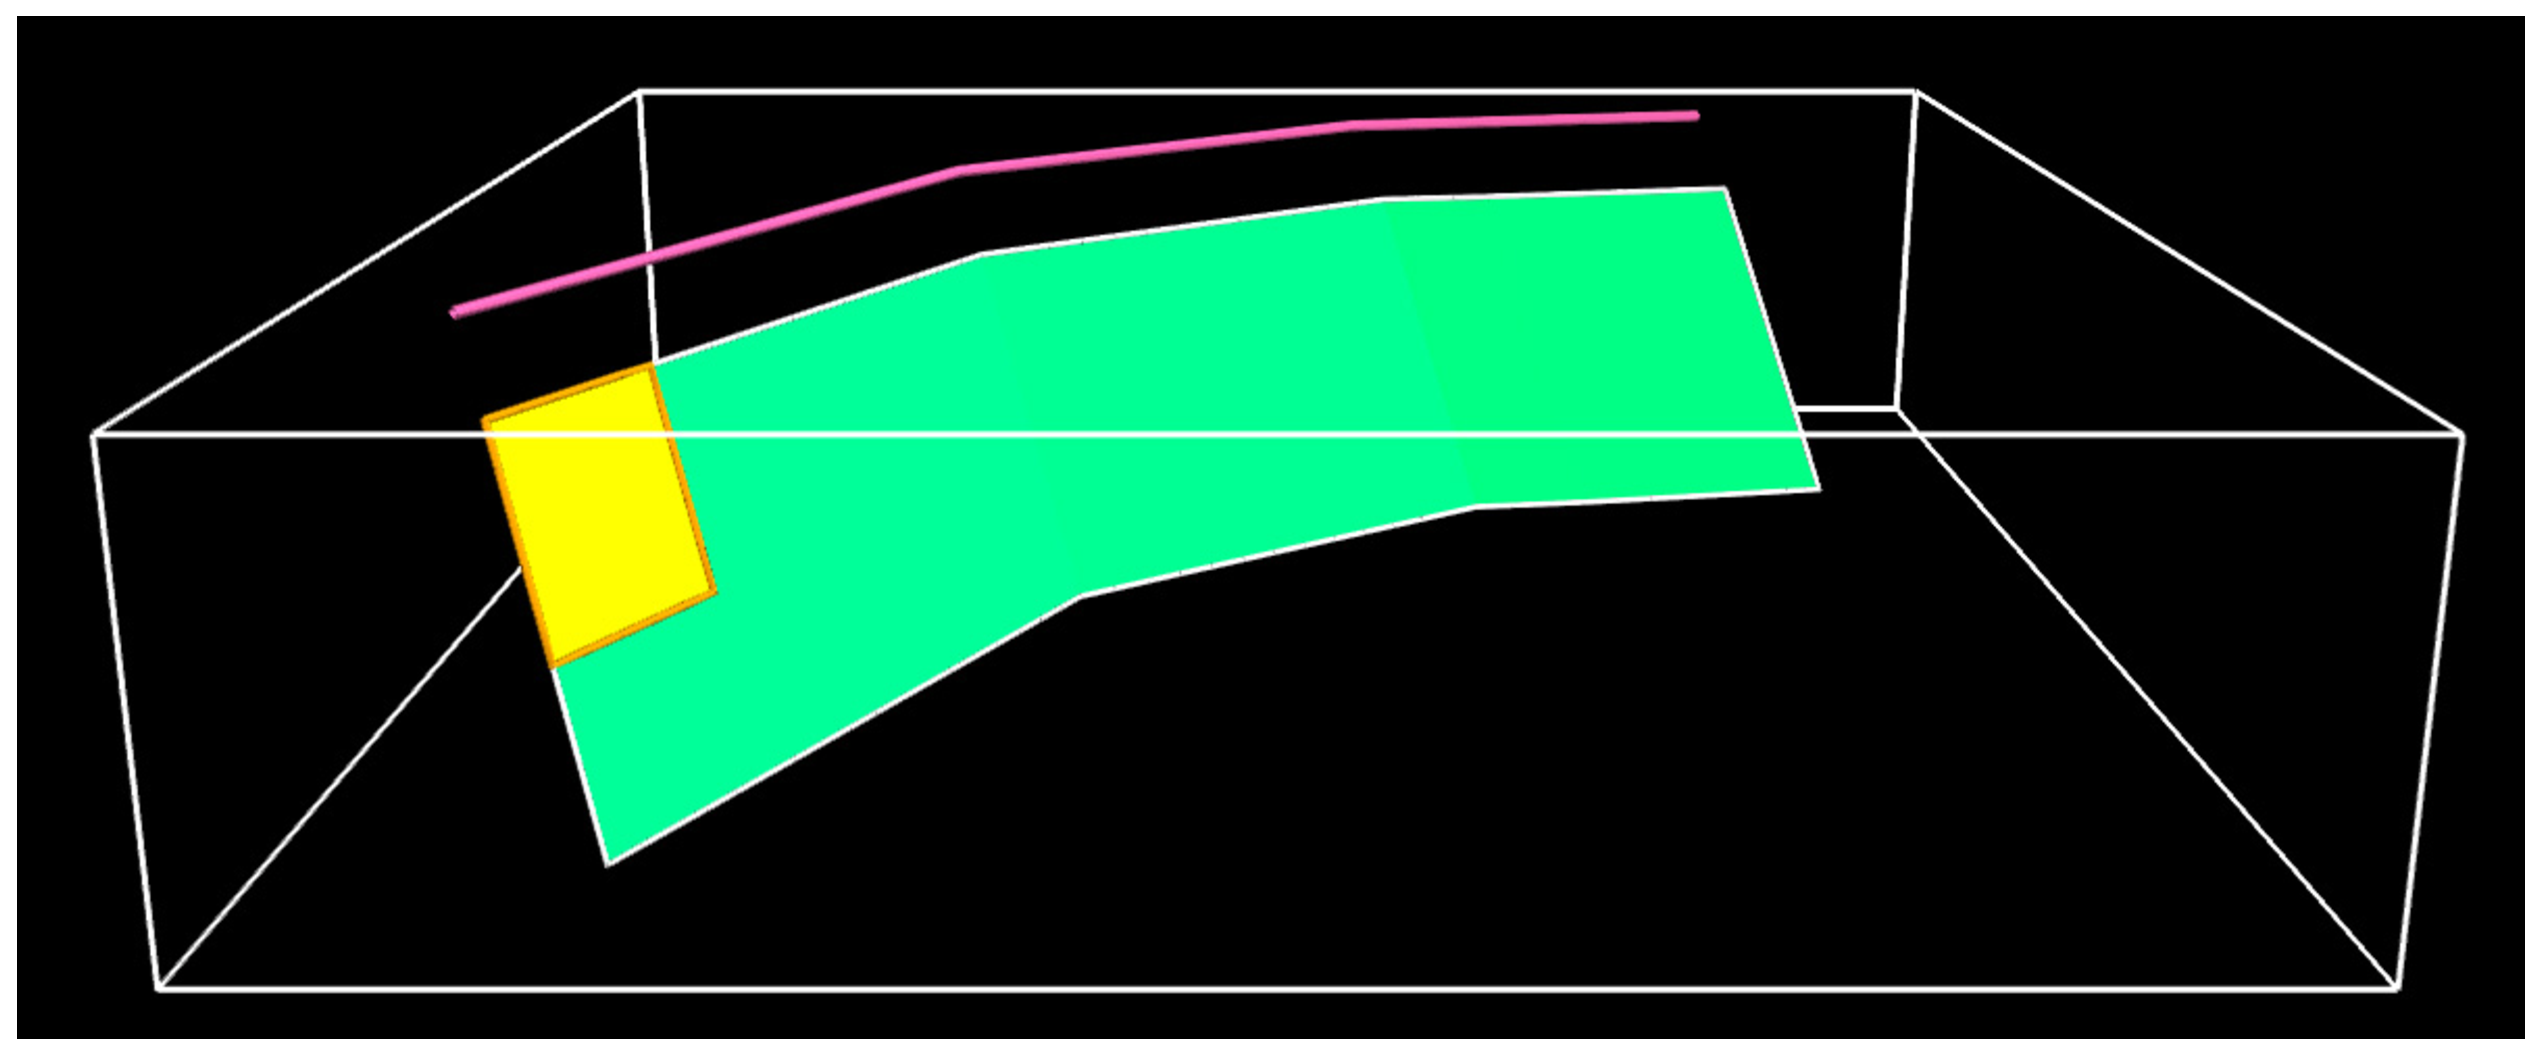
\includegraphics[width=12cm]{./figures/simpleFaultSurface.eps}
\caption{Example of simple fault source. The pink line represents the fault trace, while the green plane represents the fault surface. A single rupture (yellow plane) corresponding to a magnitude 6, with aspect ration of 1, is shown.}
\label{fig:simpleFaultSrc1}
\end{figure}
\begin{figure}[htbp]
\centering
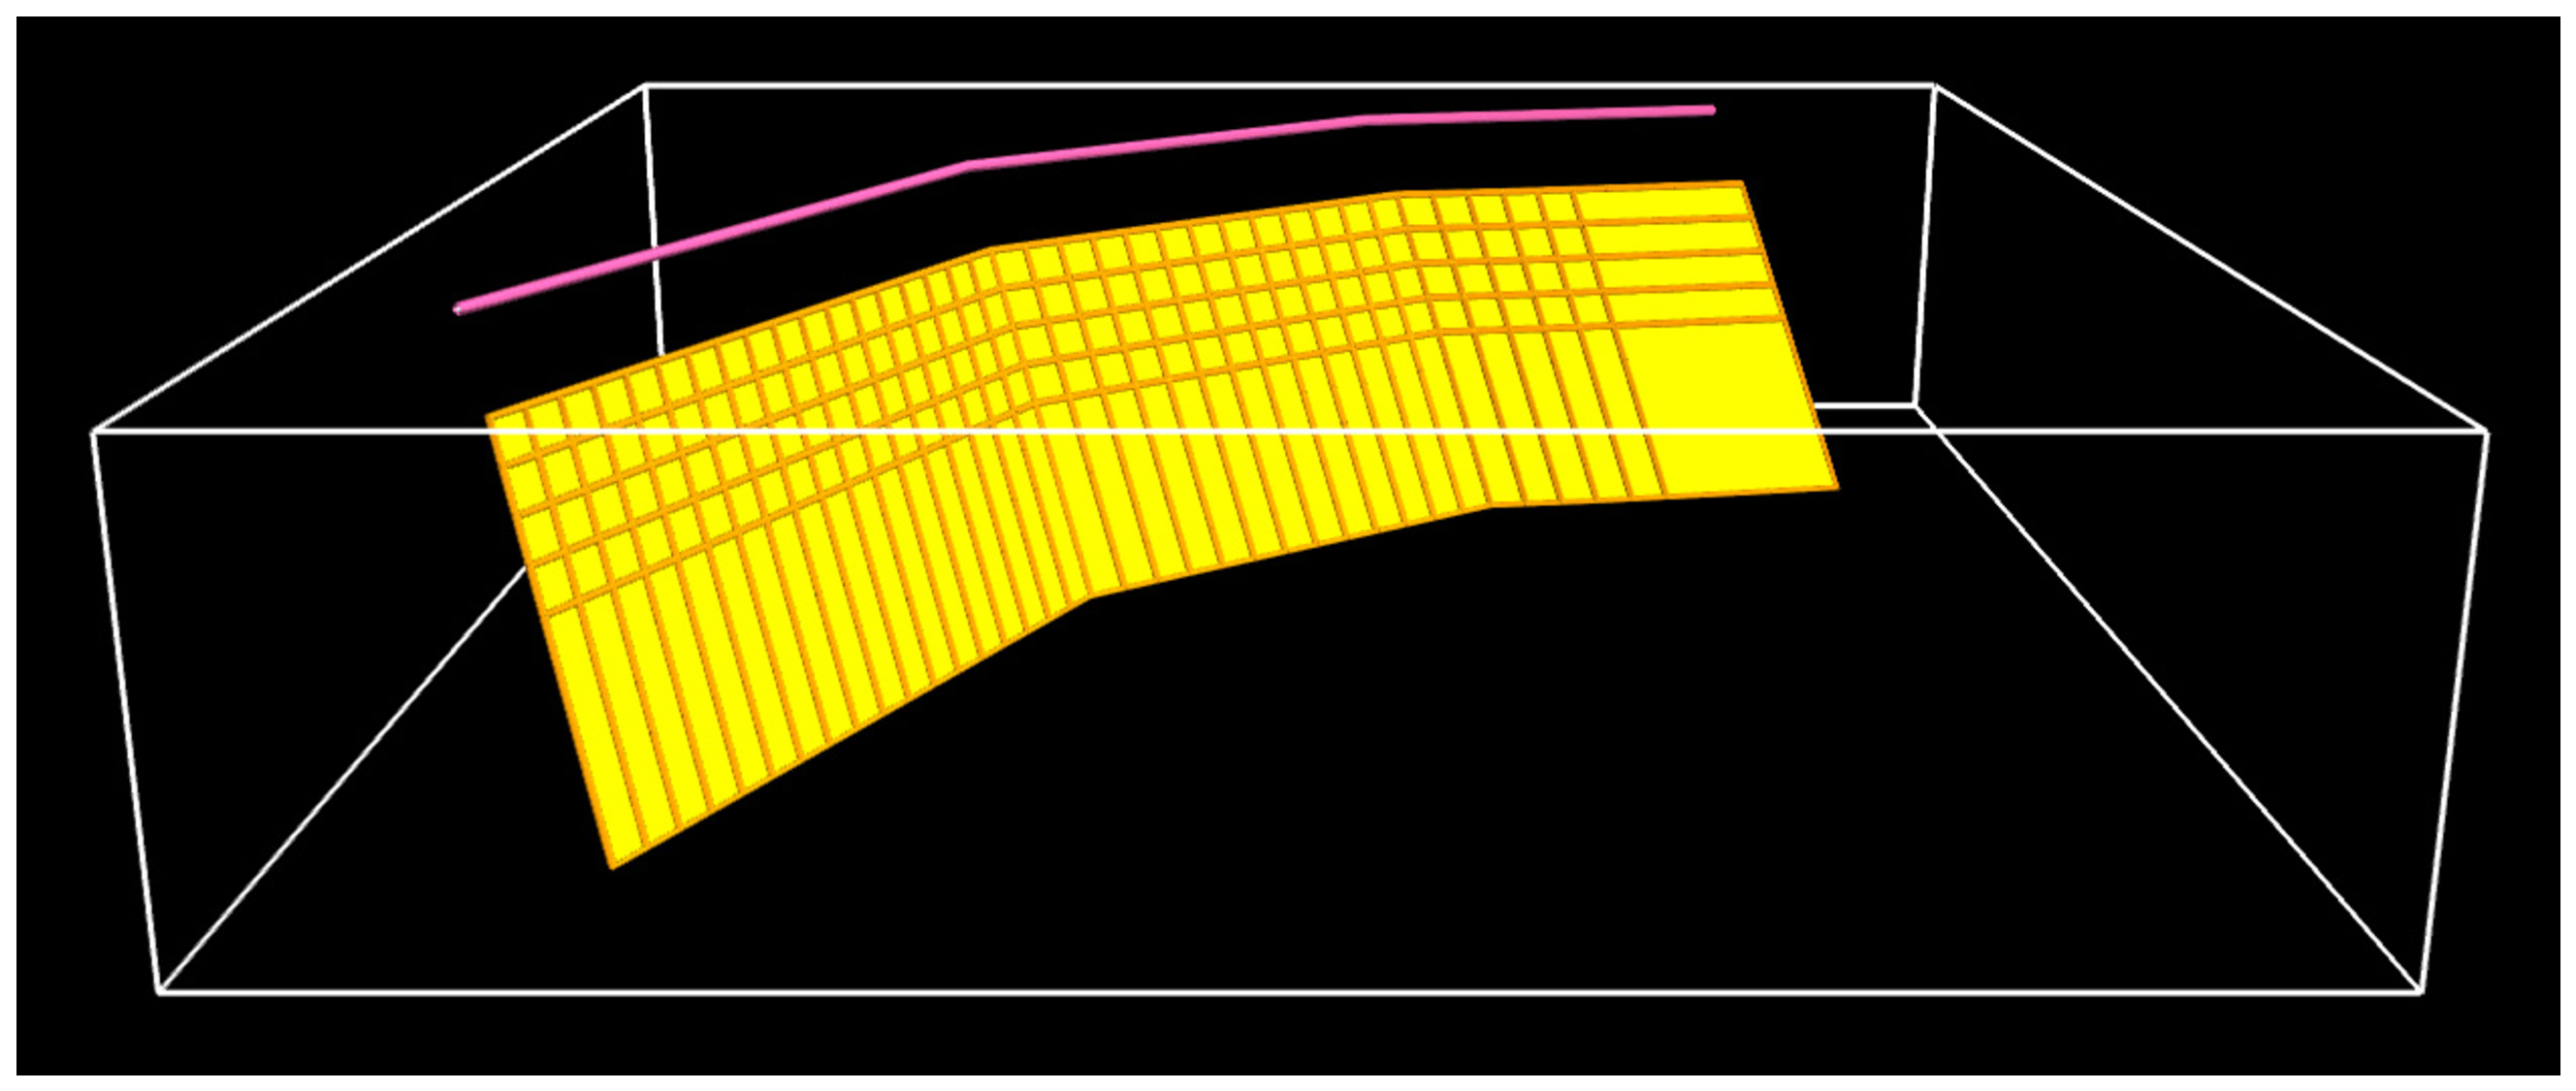
\includegraphics[width=12cm]{./figures/simpleFaultSource.eps}
\caption{Ruptures distribution in a simple fault source. To cover the entire fault surface, a rupture plane (as show in Figure \ref{fig:simpleFaultSrc1}) is shifted both along strike and dip, with an offset that is equal to the fault surface mesh spacing -- in this case 2 km.}
\label{fig:simpleFaultSrc2}
\end{figure}
\begin{figure}[htbp]
\centering
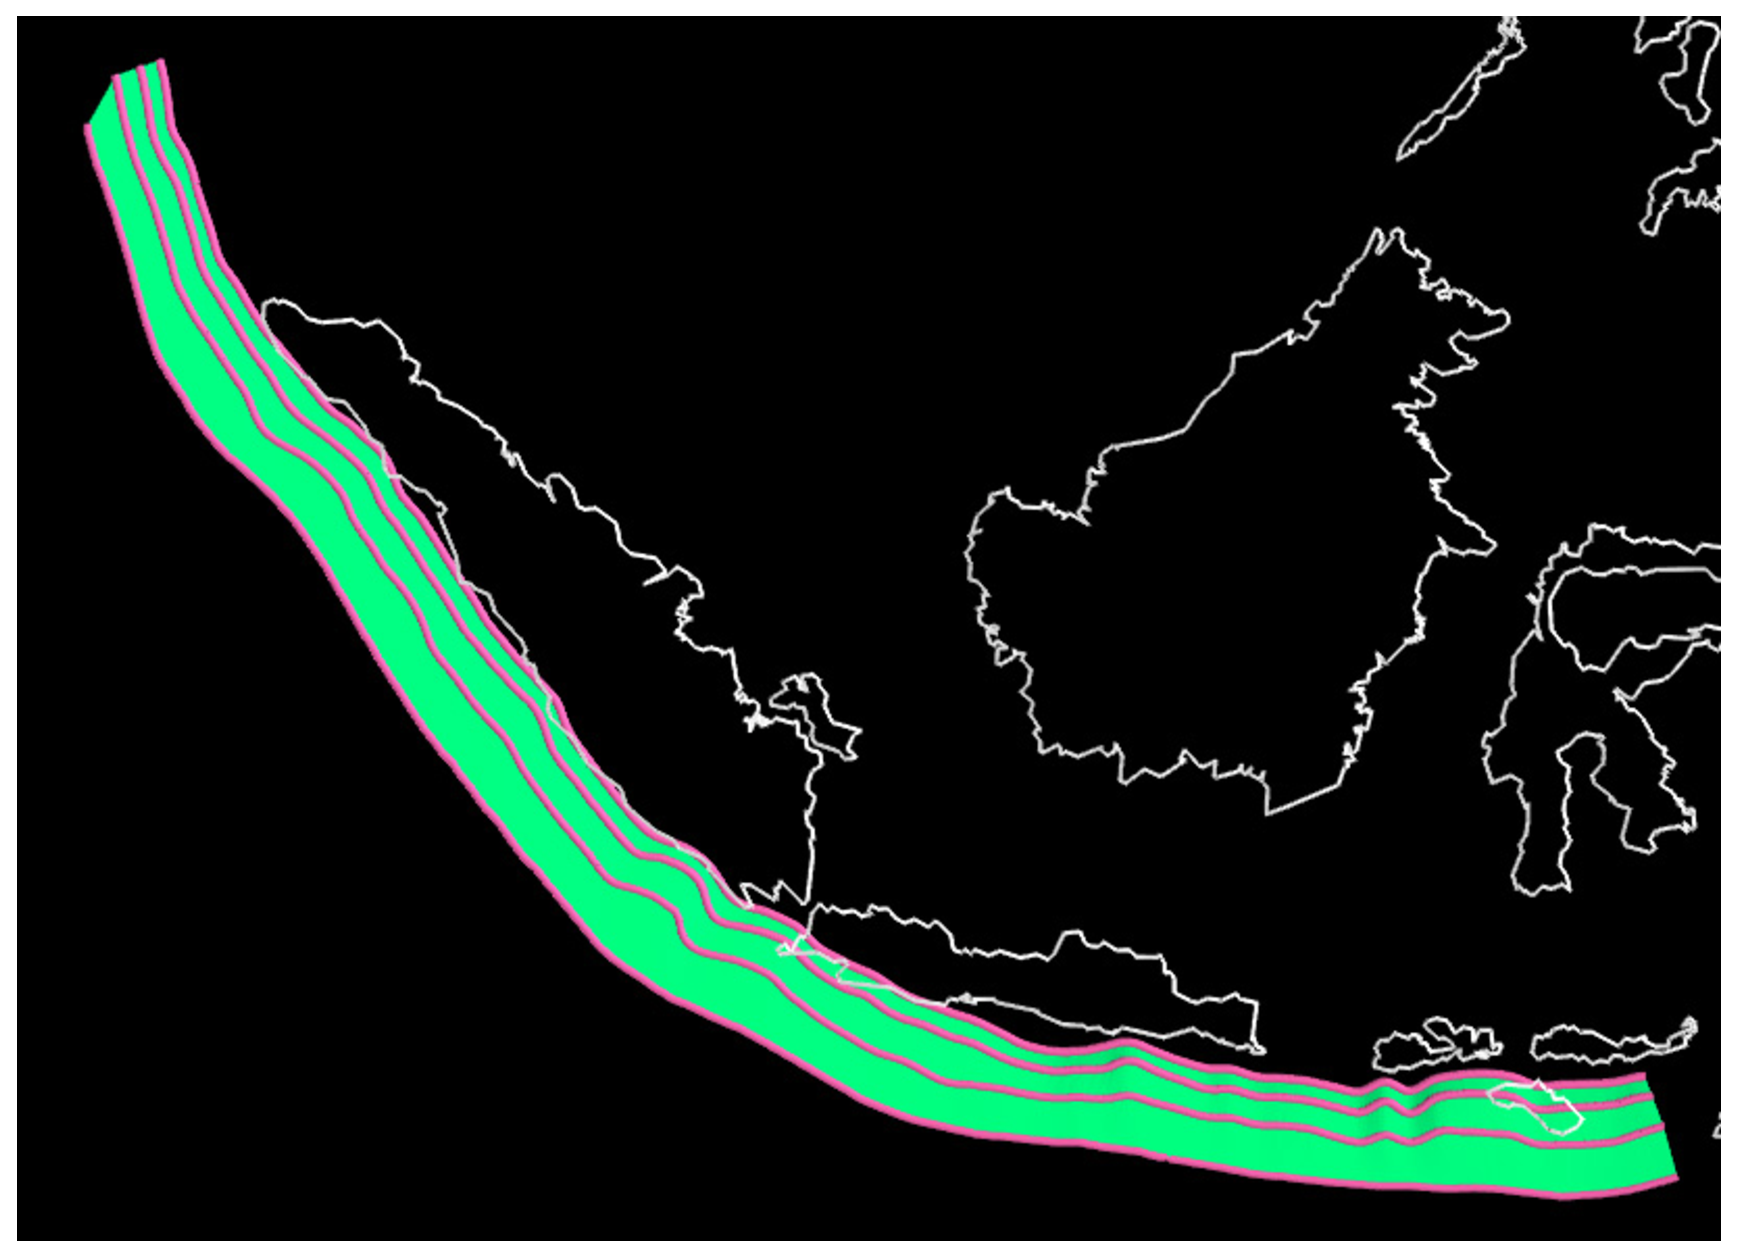
\includegraphics[width=12cm]{./figures/complexFaultSurface1.eps}
\caption{Example of complex fault source for the Sumatra-Java subduction zone as derived from the SLAB 1.0 model of \cite{hayes2012}. Starting from contour lines (pink) the fault surface (green) is computed.}
\label{fig:complexSrc}
\end{figure}
\begin{figure}[htbp]
\centering
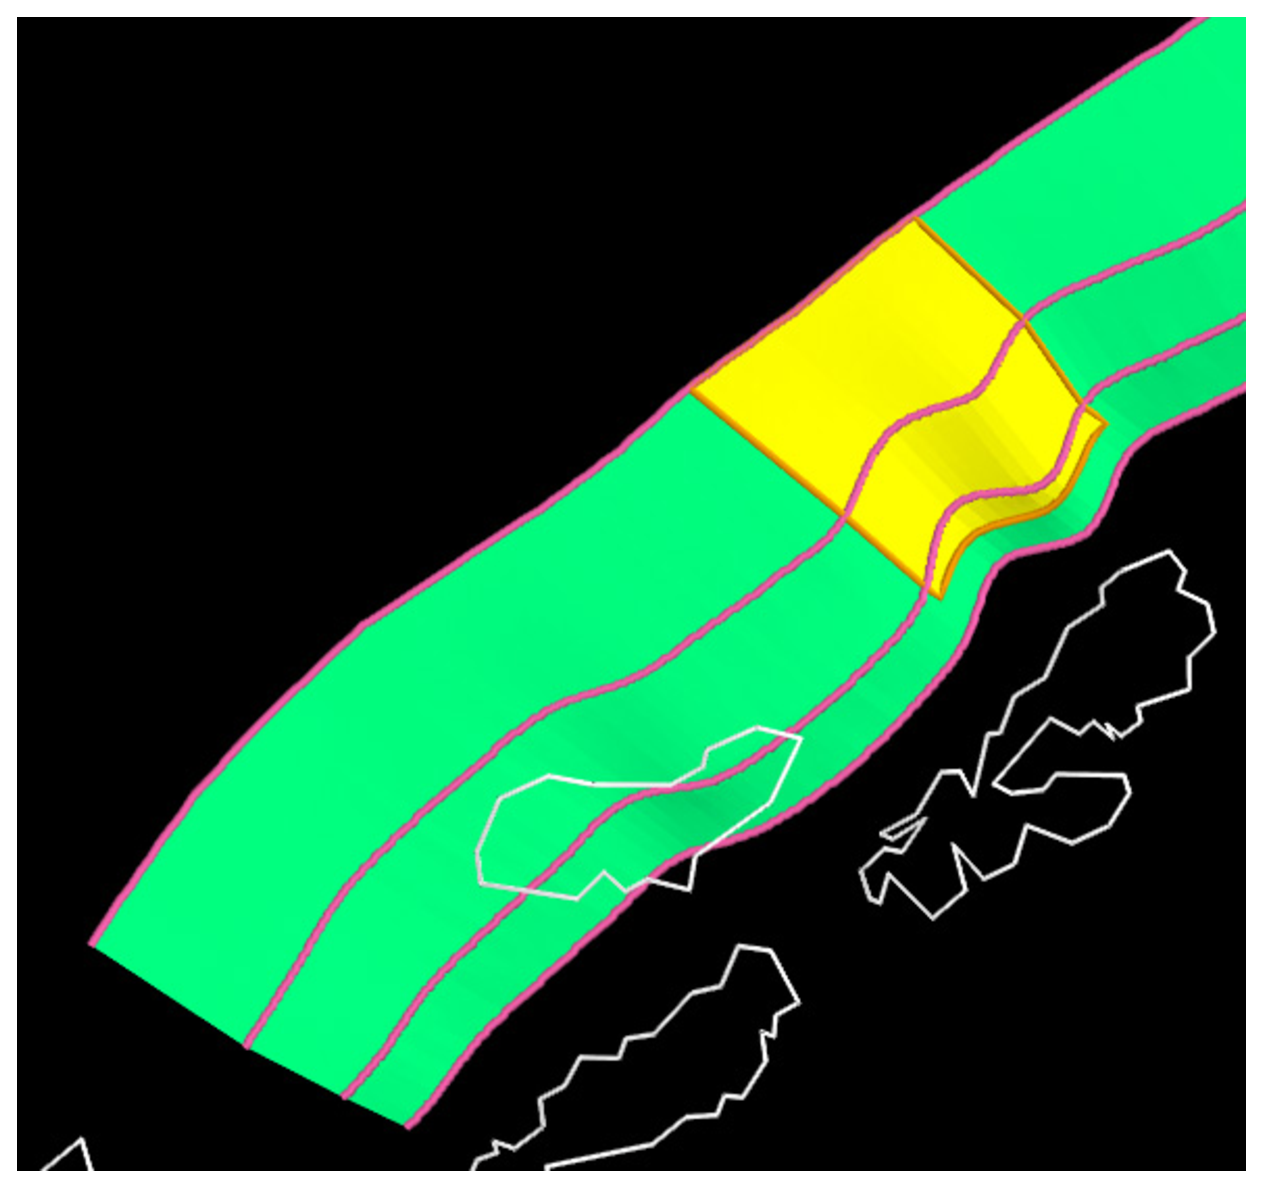
\includegraphics[width=8cm]{./figures/complexFaultSurfaceRupture.eps}
\caption{Close-up on a complex fault source rupture (M = 9, aspect ratio = 1, scaling relationship: Wells and Coppersmith 1994).}
\label{fig:complexSrcRupture}
\end{figure}

\section{Ground Shaking Intensity modeling}\label{gsim}
\setcounter{figure}{0}
NHLIB uses the term `Ground Shaking Intensity Model' to identify GMPEs and IPEs used to compute ground motion or intensity distribution at a site, given an earthquake rupture. A ground shaking intensity model is therefore designed to define a set of equations for computing mean and standard deviations (total, inter- and intra-event if available) of a Normal distribution assumed to represent the variability of an intensity measure (in case of IPEs) or of its logarithm (in case of GMPEs).\\
A ground shaking intensity model contains metadata describing proprieties such as: the tectonic region type for which the model has been derived, the supported intensity measure types (e.g. PGA, PGV, SA,...), standard deviations (e.g. total, inter- and intra-event) and component (e.g. GMRoti50, average horizontal), as well as the site (e.g. vs30, Z1pt0), rupture (e.g. top of rupture depth, focal depth, rake) and distances (e.g Rrup, Rjb, Rx) required for the mean and standard deviations calculation.\\
The implementation of a particular GMPE or IPE requires simply the definition of the metadata characterizing the model, and the equations for calculating mean and standard deviations, while all the `logic' responsible for extracting rupture and site data and performing distance calculation is encapsulated in a `base' Ground Motion Intensity Model object. This design makes the implementation of specific GMPEs/IPEs focused on the equations only, without the need of programming also those parts that relate a ground motion model with other objects in the library. In other words, introducing a new GMPE/IPE in NHLIB becomes achievable to non-professional software developer (i.e. scientists, students), given that it requires the programming of the equations only. Moreover, the NHLIB Ground Shaking Intensity Model is provided with an automatic testing procedure, which allows to validate a model as long as test data (e.g. tables) are provided in a given (ASCII) file format. This provides a built-in quality assurance procedure for the model implementation. All of this goes in the direction of simplifying the addition of user defined GMPEs/IPEs in case these are not natively present in the library.\\
A Ground Shaking Intensity Model is also designed to compute mean and standard deviation(s) for spectral acceleration periods that are not natively supported by the model, through interpolation of the equation coefficients. This is a useful feature for uniform hazard spectra calculation, and also for combining models (for instance in a logic tree) that do not share the same spectral acceleration periods.\\
 
\section{Hazard Curve calculator}\label{hcc}
\setcounter{figure}{0}
NHLIB currently provides an hazard curve calculator which assumes a Poissonian earthquake rupture forecast. The calculator computes the probability of at least one exceedance of a given intensity measure level by using the equation provided by \cite{field2003} for the case of Poissonian sources, that is:
\begin{equation}
P_{tot}(X\geq x) = 1 - \prod_{i=1}^{I} \prod_{n=1}^{N(i)} (1 - P(Rup_{i,n}))^{P(X \geq x | Rup_{i,n})}
\end{equation}
where $I$ is the total number of sources, $N(i)$ is the number of ruptures in the $i$-th source, $P(Rup_{i,n})$ is the probability of one or more occurrences of the $n$-th rupture in the $i$-th source, and  $P(X \geq x | Rup_{i,n})$ is the conditional probability of exceeding the intensity measure level $x$ given the $n$-th rupture in the $i$-th source.\\
Depending on the tectonic region type of a rupture (inherited by the source), the conditional probability of exceeding an intensity measure level is computed using the ground shaking intensity model associated to the rupture's tectonic region. In other words, the NHLIB hazard curve calculator requires as input a source model (that is a set of seismogenic sources) and a set of ground shaking intensity models, one for each tectonic region type considered in a source model.\\
The calculator provides also a filtering mechanism to ignore sources and ruptures that are more than a user defined distance far from the sites considered. The filtering mechanism is meant as an optimization mechanism (to ignore those sources that being too far would contribute little to the hazard in a given site), but also to take into account the distance range for which ground shaking intensity models are valid. GMPEs/IPEs usually defines their own range of validity, however given the need of combining different models in the same calculation, the definition of the distance range to consider in a calculation is done explicitly by the user.

\section{PEER Tests}\label{peer}
\setcounter{figure}{0}
NHLIB currently implements 4 PEER Tests (\cite{thomas2010}) as `Acceptance Tests' for the library. The tests implemented are:
\begin{itemize}
\item Set 1 Case 2:  Vertical fault with single rupture smaller than fault plane
\item Set 1 Case 5:  Vertical fault with truncated Gutenberg-Richter distribution ($M_{min}=5$ and $M_{max}=6.5$)
\item Set 1 Case 10: Area Source with ruptures at fixed depth of 5 km and truncated Gutenberg-Richter distribution ($M_{min}=5$ and $M_{max}=6.5$)
\item Set 1 Case 11: Area source with ruptures distributed between 5 km and 10 km and truncated Gutenberg-Richter distribution ($M_{min}=5$ and $M_{max}=6.5$)
\end{itemize}
Figures \ref{fig:case2site1} to \ref{fig:case11site1} show comparisons between hazard curves, for a single site, as computed by NHLIB and as defined in the PEER Report. We can notice a very good agreement for the test cases 2 and 5 (that is for a simple fault), while we see a divergence between the computed and the expected curves for the test 10 and 11 (that is for the area source). The divergence is visible for the higher ground motion values. This can be explained by the fact that the reference solutions for the area test cases assume ruptures to be modeled as points (as written in the report, pag. 14: ''Use 1 km grid spacing of point sources or small faults to simulate uniform distribution"). NHLIB can currently model ruptures only as extended. Indeed, by modifying the PEER magnitude area scaling relationship to provide a very small area (0.1 squared km) independently of the magnitude value, the fit between the computed curves and the expected ones improves significantly (see Figures \ref{fig:case10site1point} and \ref{fig:case11site1point}) 
\begin{figure}[htbp]
\centering
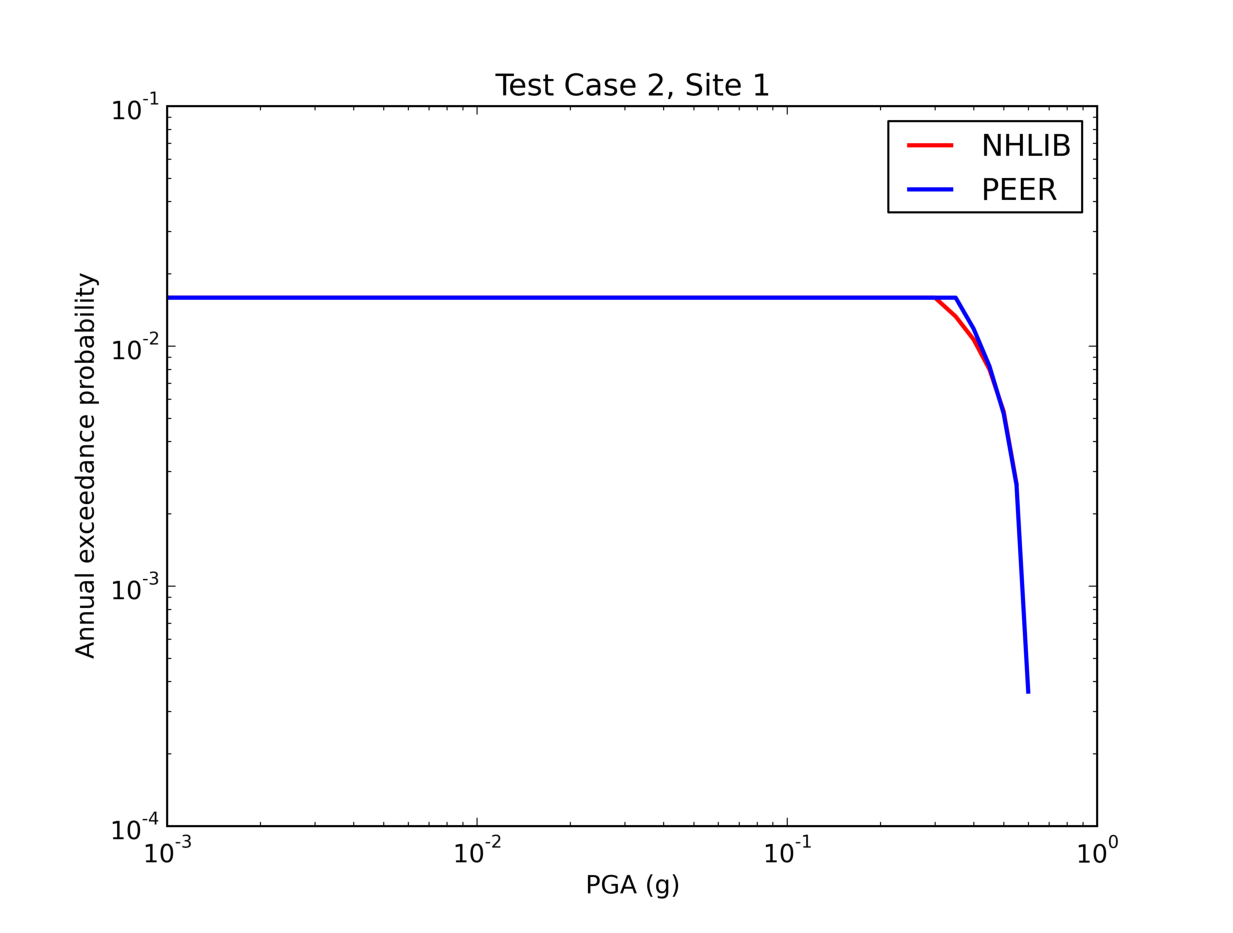
\includegraphics[width=12cm]{./figures/Case2Site1.eps}
\caption{PEER test case 2 on site 1.}
\label{fig:case2site1}
\end{figure}
\begin{figure}[htbp]
\centering
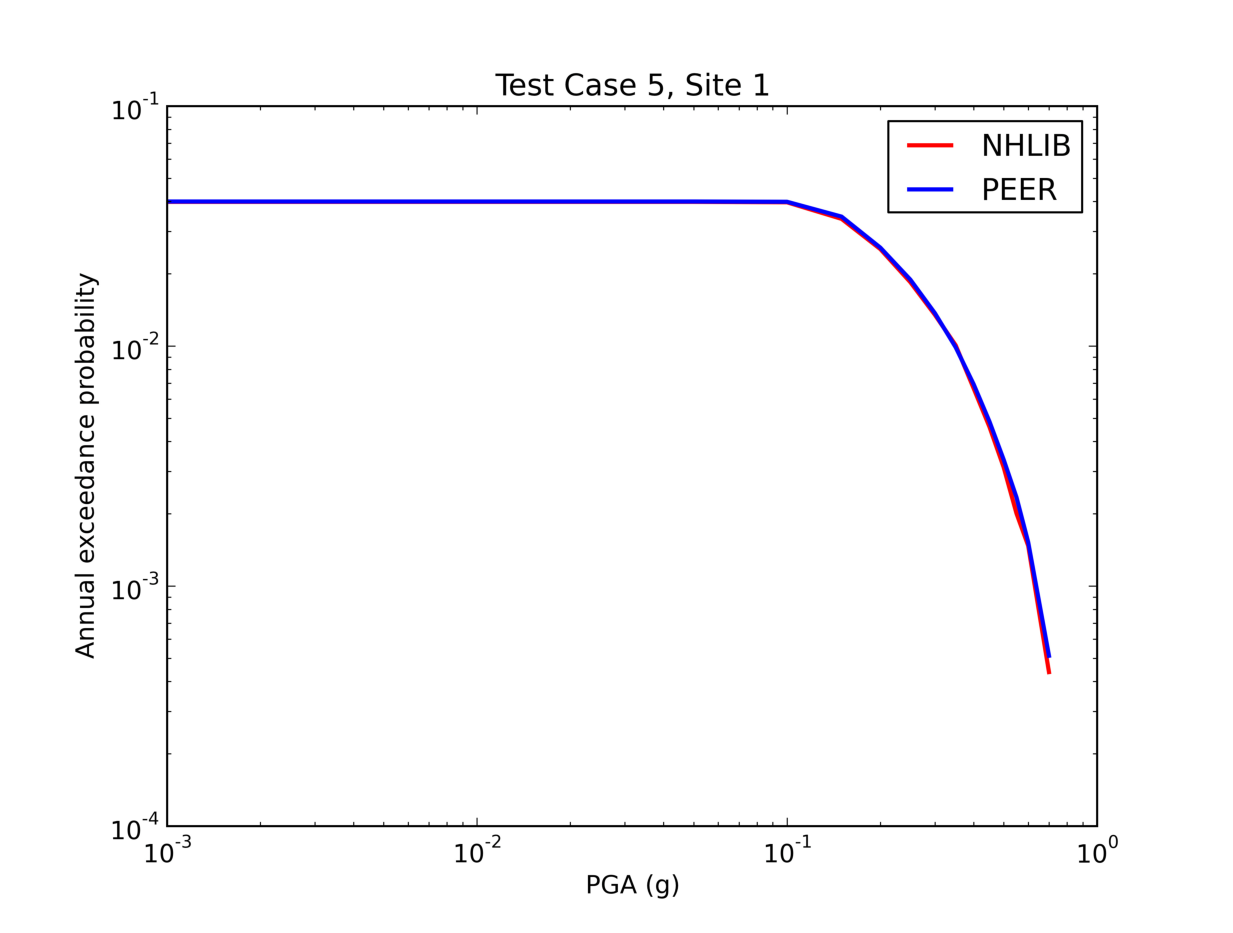
\includegraphics[width=12cm]{./figures/Case5Site1.eps}
\caption{PEER test case 5 on site 1.}
\label{fig:case5site1}
\end{figure}
\begin{figure}[htbp]
\centering
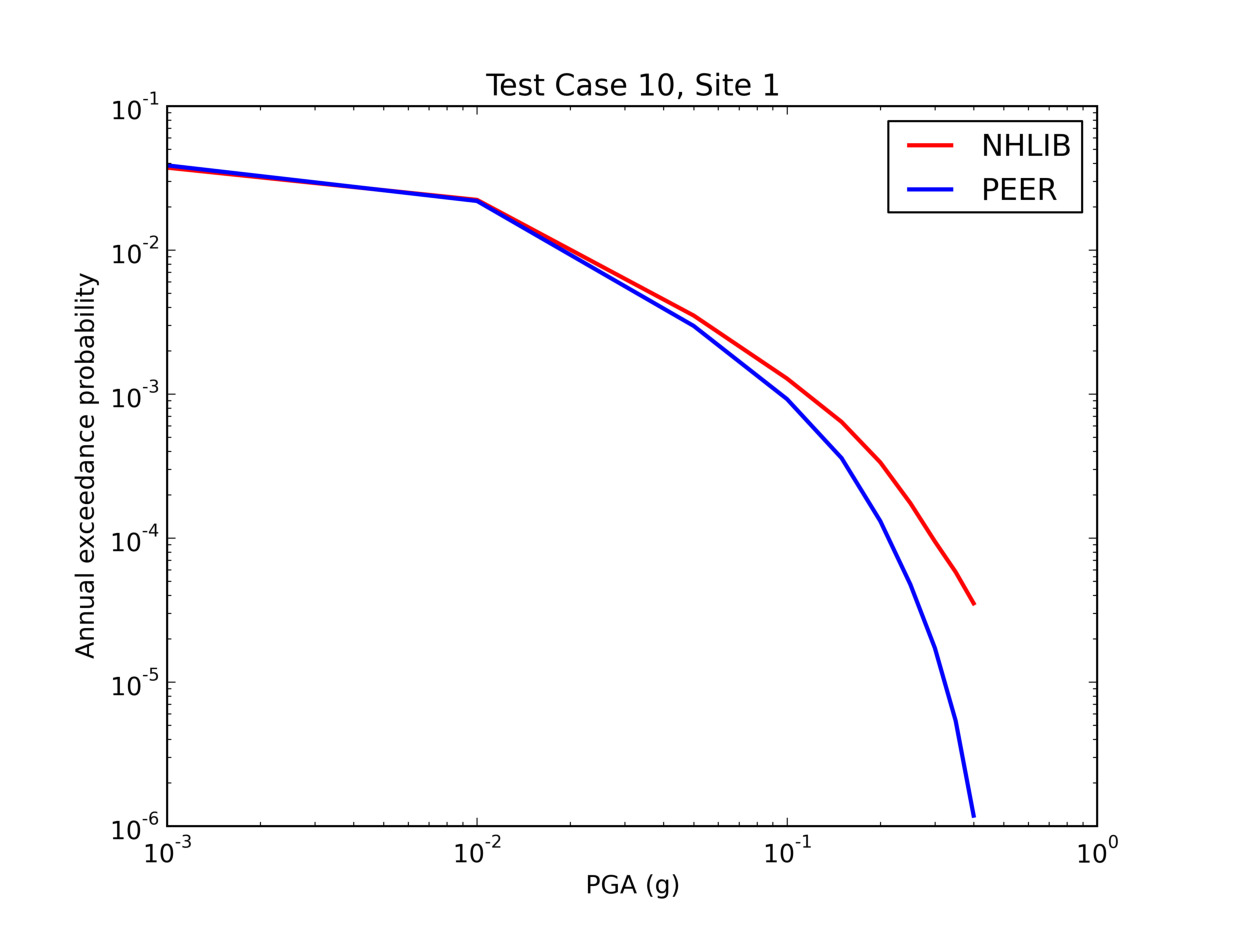
\includegraphics[width=12cm]{./figures/Case10Site1.eps}
\caption{PEER test case 10 on site 1.}
\label{fig:case10site1}
\end{figure}
\begin{figure}[htbp]
\centering
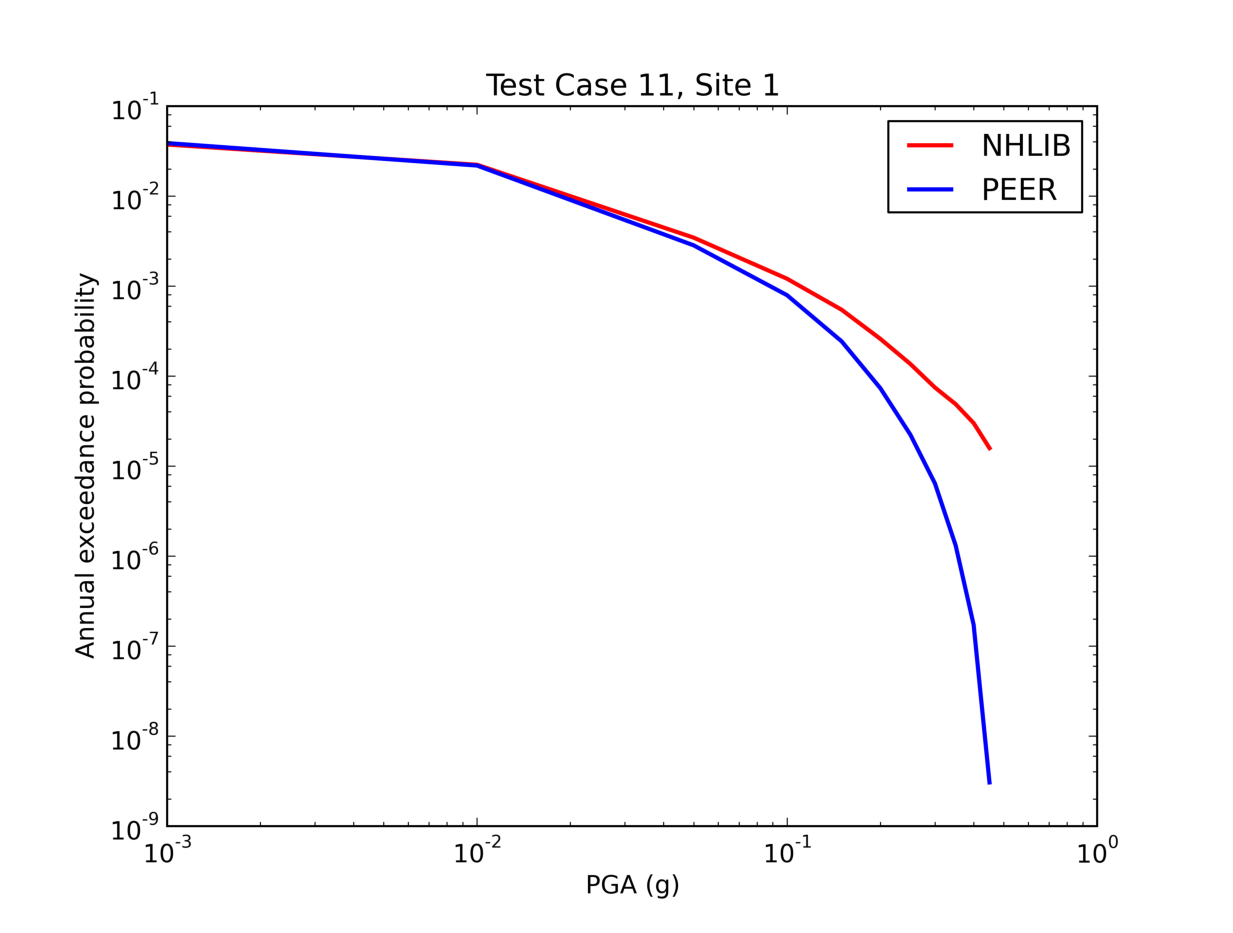
\includegraphics[width=12cm]{./figures/Case11Site1.eps}
\caption{PEER test case 11 on site 1.}
\label{fig:case11site1}
\end{figure}
\begin{figure}[htbp]
\centering
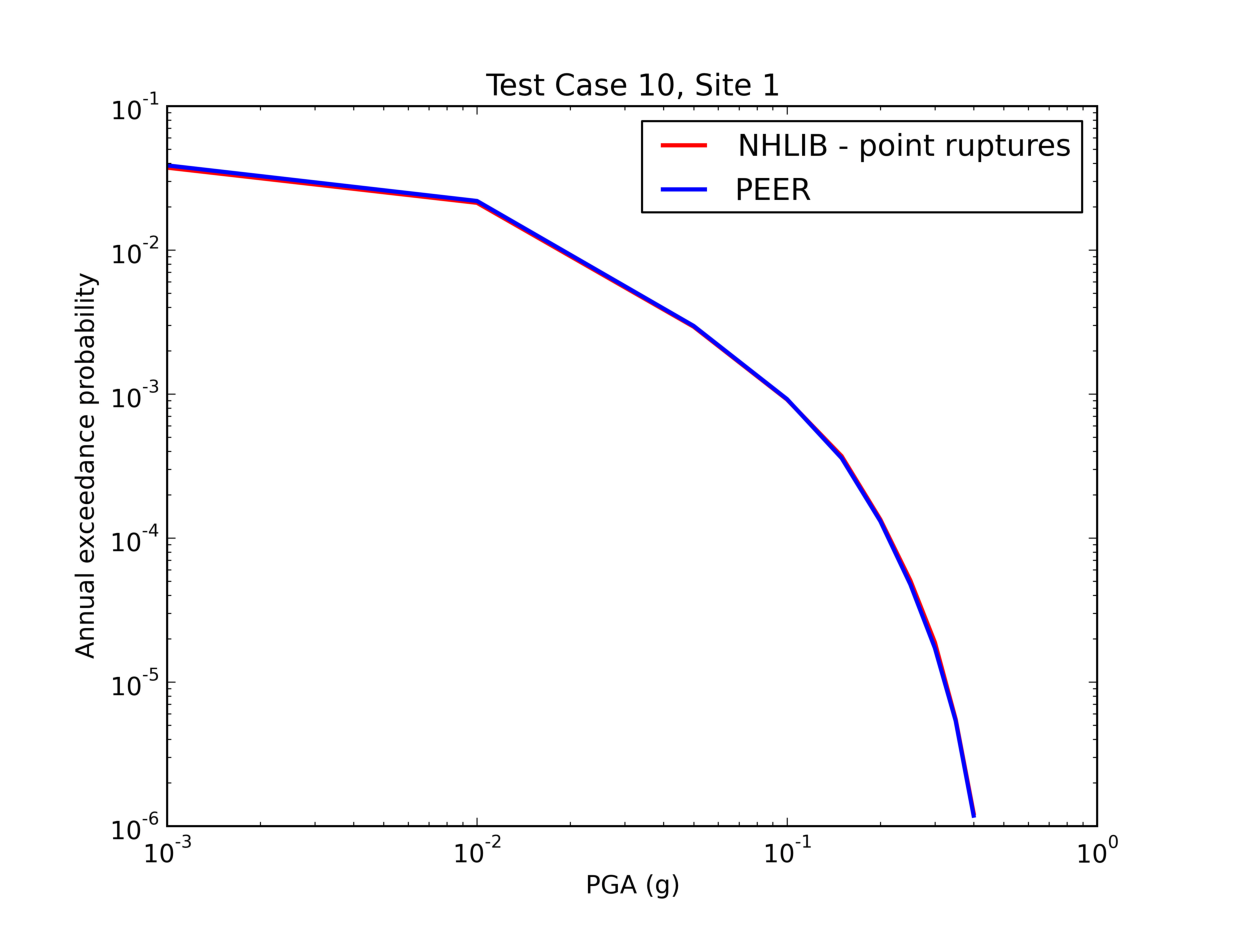
\includegraphics[width=12cm]{./figures/Case10Site1_point.eps}
\caption{PEER test case 10 on site 1 assuming point ruptures.}
\label{fig:case10site1point}
\end{figure}
\begin{figure}[htbp]
\centering
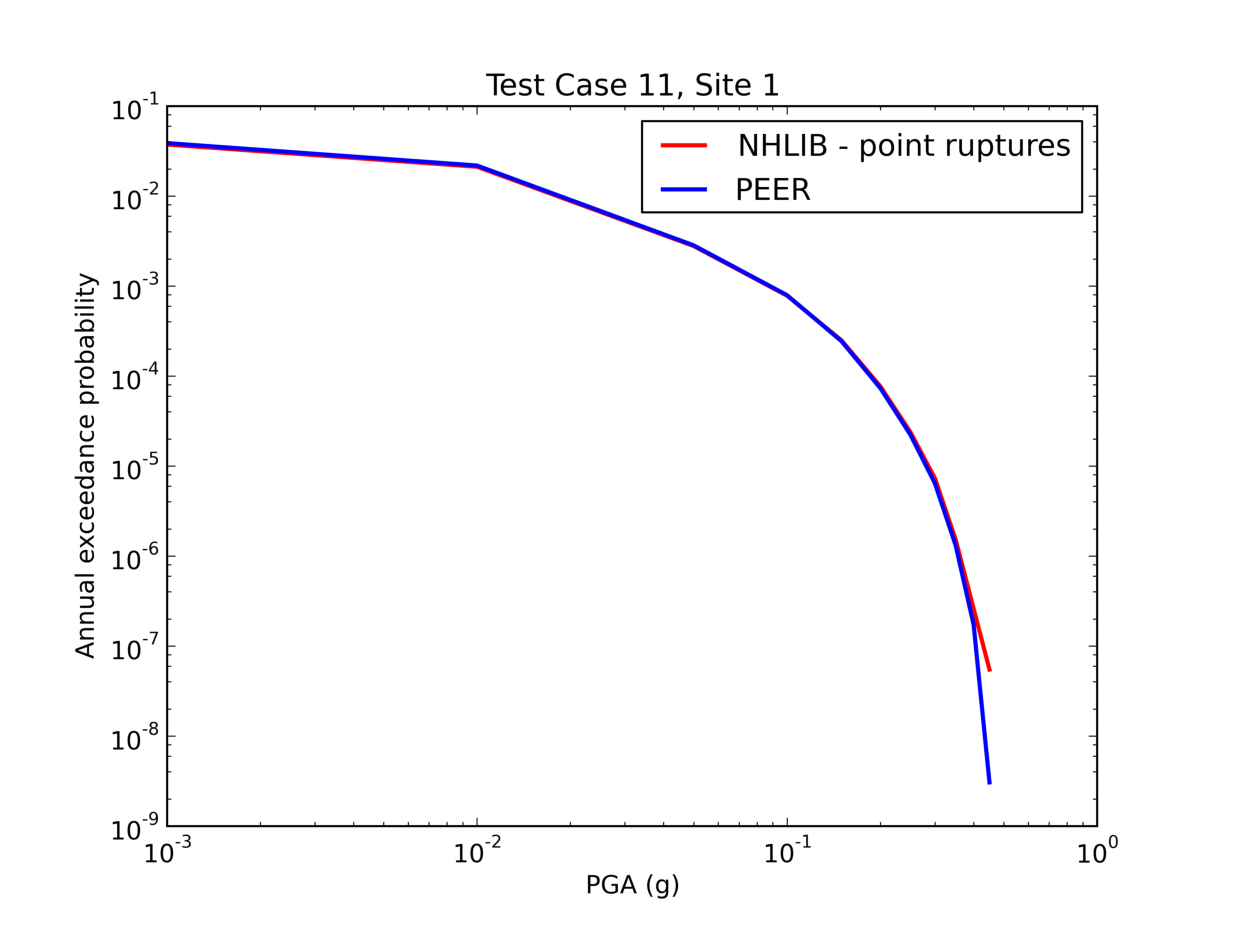
\includegraphics[width=12cm]{./figures/Case11Site1_point.eps}
\caption{PEER test case 11 on site 1 assuming point ruptures.}
\label{fig:case11site1point}
\end{figure}


\section{Performances}\label{performances}
\setcounter{figure}{0}
As described in section \ref{hcc}, the calculation of an hazard curve on a site depends mainly on how many ruptures each source defines. Greater is the number of ruptures, greater is the time spent for the rupture creation, and greater is the number of times probabilities of exceedance need to be computed (and therefore ground shaking intensity models evaluated). Number of ruptures, and number of sites for which hazard curves need to be computed affect mostly the performances of hazard curves calculations.\\
Figure \ref{fig:ctsites} shows how the computation time varies with number of sites considering different sets of sites. In this analysis ruptures are created from a single area source, and different sets of ruptures are obtained by considering different discretization intervals of the area source. As expected, as the number of ruptures increases, also the computation time increases. However, we also observe that the number of sites starts to play a role in increasing the computation time only above about 1000 sites. Above this value, the computation time increases linearly with the number of sites (the plot shows a power grow because of a log-linear scale).The main reason for this behaviour is the vectorization of ground shaking calculations over sites. That is, given an earthquake rupture, ground shaking (mean and standard deviations) at a set of sites are computed in a single function call, rather than by multiple function calls through a loop.\\
Figure \ref{fig:ctsiteopt} shows instead how the performances of the engine improved during the development of the library. The magenta line represent performances with the initiali implementation of the hazard curve calculator. The vectorization of distance calculations and the employment of analytical approaches for calculating rupture to sites distances helped in reducing computation time. However the major speed-up was obtained by vectorizing ground shaking intensity model calculations (that is mean and standard deviation calculation). Additional improvement was obtained by optimizing the rupture creation in area sources: that is ruptures are created only once in a node inside the area boundary, and then simply translated to the remaining nodes, rather then recreated every time at each node.\\
The presented tests have been run on a AMD Opteron 6174, 2.2 GHz processor and no significant RAM usage has been identified (RAM usage of the process running hazard curve calculation never exceeded 50 Mb).\\
\begin{figure}[htbp]
\centering
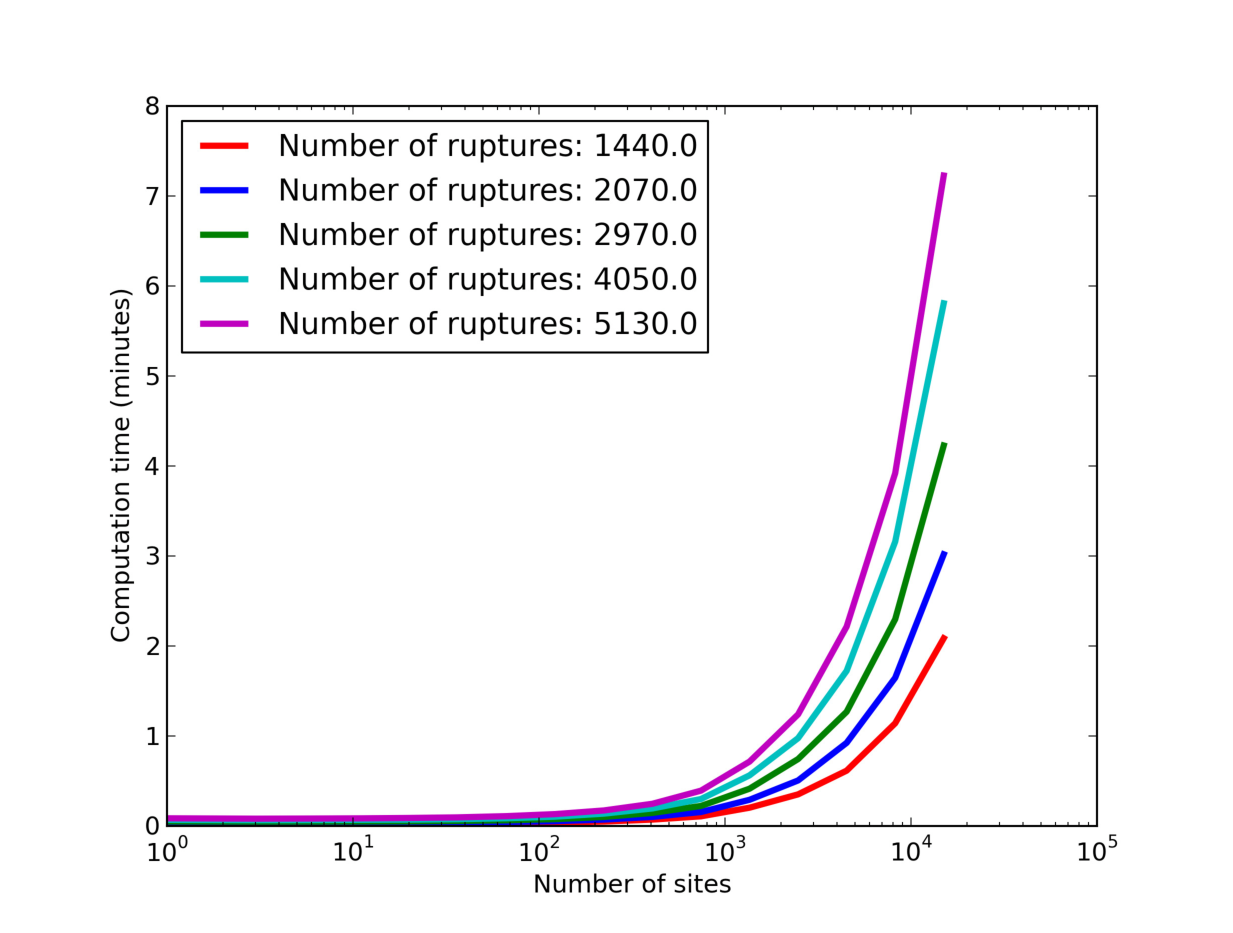
\includegraphics[width=14cm]{./figures/ComputationTimeVsSites.eps}
\caption{Computation time versus number of sites for different set of ruptures.}
\label{fig:ctsites}
\end{figure}
\begin{figure}[htbp]
\centering
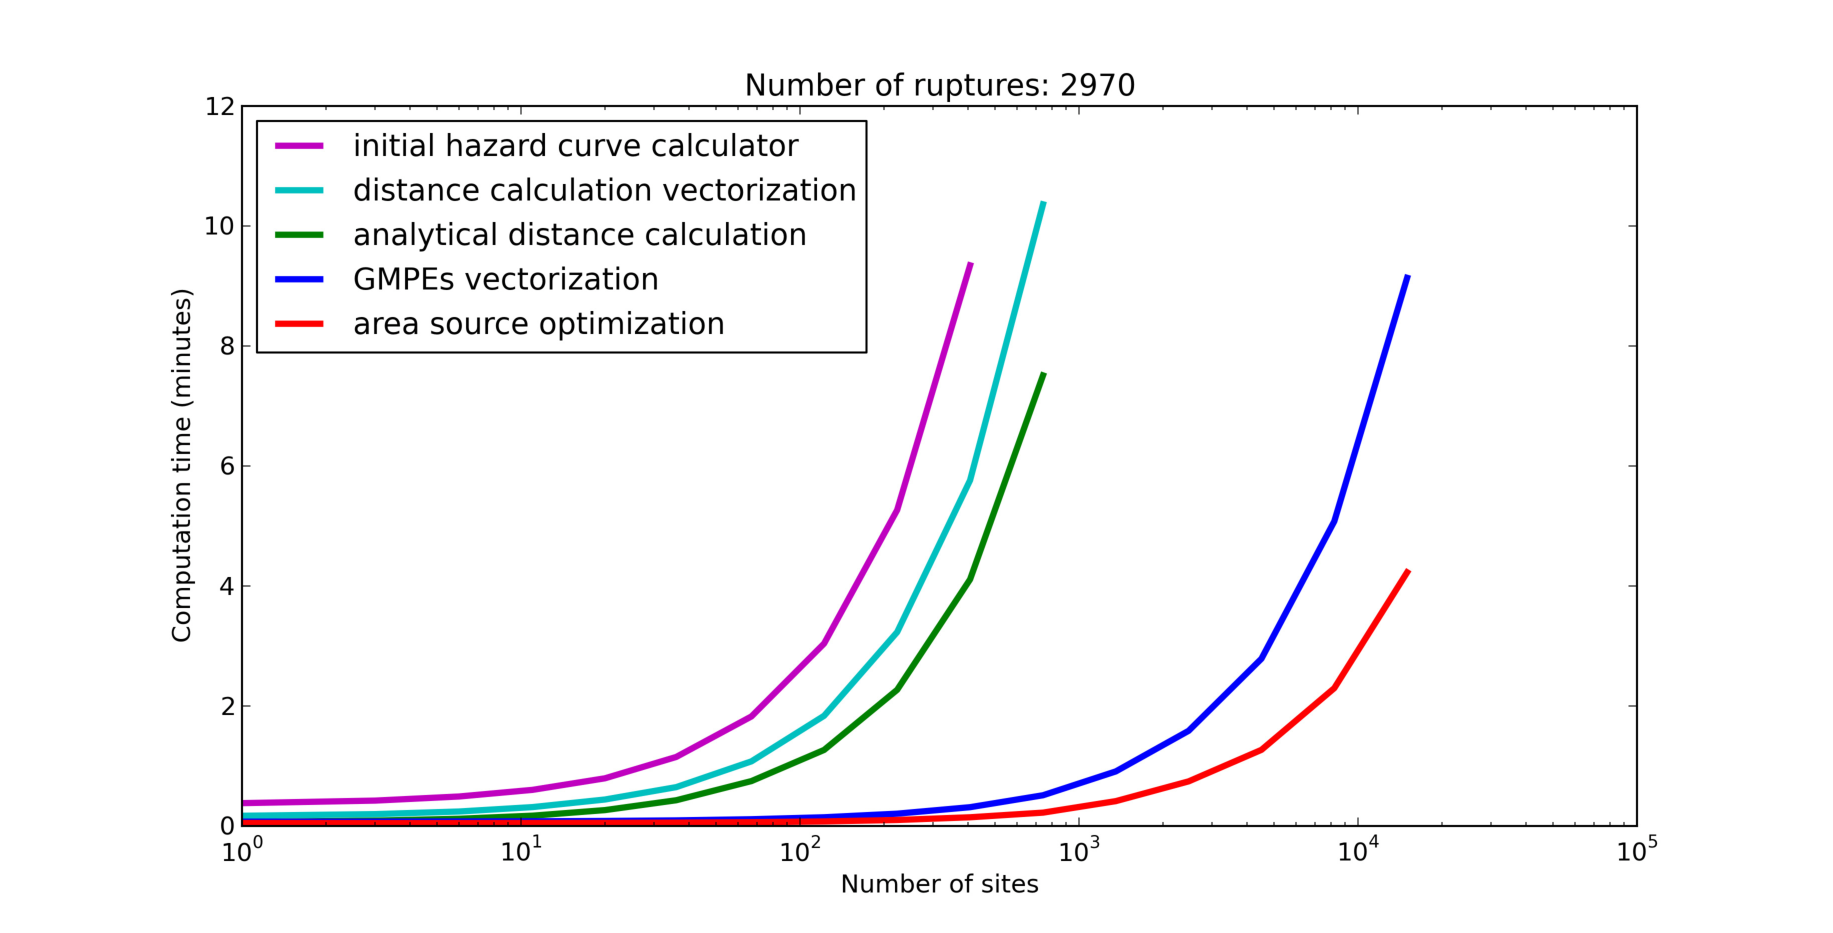
\includegraphics[width=16cm]{./figures/ComputationVsSitesVsOptimizations.eps}
\caption{Computation time versus sites for different optimizations.}
\label{fig:ctsiteopt}
\end{figure}

\section{Conclusions}\label{conclusions}
\setcounter{figure}{0}
NHLIB provides the capability to model seismicity according to the four source typologies (point, area, simple fault and complex fault) that are currently used by OpenQuake. In all source typologies, ruptures are modeled as 3D surfaces. Distance metrics which require extended ruptures (like closest distance to rupture or Joyner-Boore distance) can be therefore honored. Point and area sources allow distributing ruptures over multiple depth (in case an hypocentral depth distribution is available) and also over multiple nodal planes (useful to simulate ruptures oriented over multiple azimuths).\\
Ground shaking intensity models can be both GMPEs or IPEs, and can provide ground motion distribution parameters also at periods that are not supported by the original model by interpolating equation coefficients. Ground motion parameters can be obtained in a vectorized fashion therefore allowing efficient processing of large set of sites.\\
NHLIB currently provides an hazard curve calculator which assumes a Poissonian earthquake rupture forecast. A first set of optimizations has been done, which allowed to improve significantly the calculation efficiency. For the same computation time, the current hazard curve calculator can process about 100 times more sites than the initial implementation of the calculator.\\
NHLIB will provide also calculators for stochastic event set generation, ground motion field calculation -- with spatial correlation, and for disaggregation analysis. A more clear understanding of the NHLIB performances will come once the library will be tested with realistic PSHA models and also integrated in OpenQuake, which will provide an additional speed-up thanks to the capability of distributing calculations over multiple processes running in a parallel fashion.\\ 
NHLIB has been developed since the very beginning following a 'Test Driven Development' strategy. This means that, as much as possible, every function in the library is tested against one or more use cases, which are meant to check the correctness of the function but also that it fails in a predictable way when incomplete or invalid data are passed in. By running a test coverage analysis over the library it's possible to quantify the test coverage in each module (see Figure \ref{fig:testcoverage}). At the current stage of development, all modules of NHLIB have a full test coverage. In other words, this means that every line of code is executed at least once by a test case. Such a comprehensive monitoring gives an high level of confidence in the results produced by the library (even if it does not necessarily guarantee that no bugs exists, because functions may not have been tested against the full range of possible input data), but more importantly puts the library under a controlled environment which makes introducing new features or optimizations an easier and safer task.\\
\begin{figure}[htbp]
\centering
\begin{Verbatim}[frame=single, commandchars=\\\{\}, fontsize=\scriptsize,samepage=true]
Name                              Stmts   Miss  Cover   Missing
---------------------------------------------------------------
nhlib                                 2      0   100%   
nhlib.calc                            2      0   100%   
nhlib.calc.hazard_curve              17      0   100%   
nhlib.const                          23      0   100%   
nhlib.geo                            10      0   100%   
nhlib.geo._utils                     93      0   100%   
nhlib.geo.geodetic                   99      0   100%   
nhlib.geo.line                       68      0   100%   
nhlib.geo.mesh                      206      0   100%   
nhlib.geo.nodalplane                 19      0   100%   
nhlib.geo.point                      36      0   100%   
nhlib.geo.polygon                    75      0   100%   
nhlib.geo.surface                     4      0   100%   
nhlib.geo.surface.base               31      0   100%   
nhlib.geo.surface.complex_fault      43      0   100%   
nhlib.geo.surface.planar            106      0   100%   
nhlib.geo.surface.simple_fault       50      0   100%   
nhlib.gsim                            1      0   100%   
nhlib.gsim.base                     137      0   100%   
nhlib.gsim.chiou_youngs_2008         56      0   100%   
nhlib.gsim.sadigh_1997               76      0   100%   
nhlib.imt                            31      0   100%   
nhlib.mfd                             3      0   100%   
nhlib.mfd.base                       32      0   100%   
nhlib.mfd.evenly_discretized         20      0   100%   
nhlib.mfd.truncated_gr               64      0   100%   
nhlib.pmf                             9      0   100%   
nhlib.scalerel                        3      0   100%   
nhlib.scalerel.base                  19      0   100%   
nhlib.scalerel.peer                   7      0   100%   
nhlib.scalerel.wc1994                40      0   100%   
nhlib.site                           37      0   100%   
nhlib.source                          6      0   100%   
nhlib.source.area                    29      0   100%   
nhlib.source.base                    22      0   100%   
nhlib.source.complex_fault           60      0   100%   
nhlib.source.point                   68      0   100%   
nhlib.source.rupture                 26      0   100%   
nhlib.source.simple_fault            54      0   100%   
nhlib.tom                             9      0   100%   
---------------------------------------------------------------
TOTAL                              1693      0   100%   
----------------------------------------------------------------------
Ran 372 tests in 124.009s
\end{Verbatim}
\caption{Test coverage for all NHLIB modules. `Stmts' represents the number of lines of code tested, `Miss' defines the number of lines not tested, and `Cover' gives the percentage of test coverage.}
\label{fig:testcoverage}
\end{figure}

\bibliographystyle{apalike}
\bibliography{./Bibliography/hazard}

\end{document}
